\section{Introduction}
Ce TP va vous apprendre à créer une page HTML basique, puis à la personnaliser
avec du CSS. Vous devriez obtenir le résultat suivant :

\begin{center}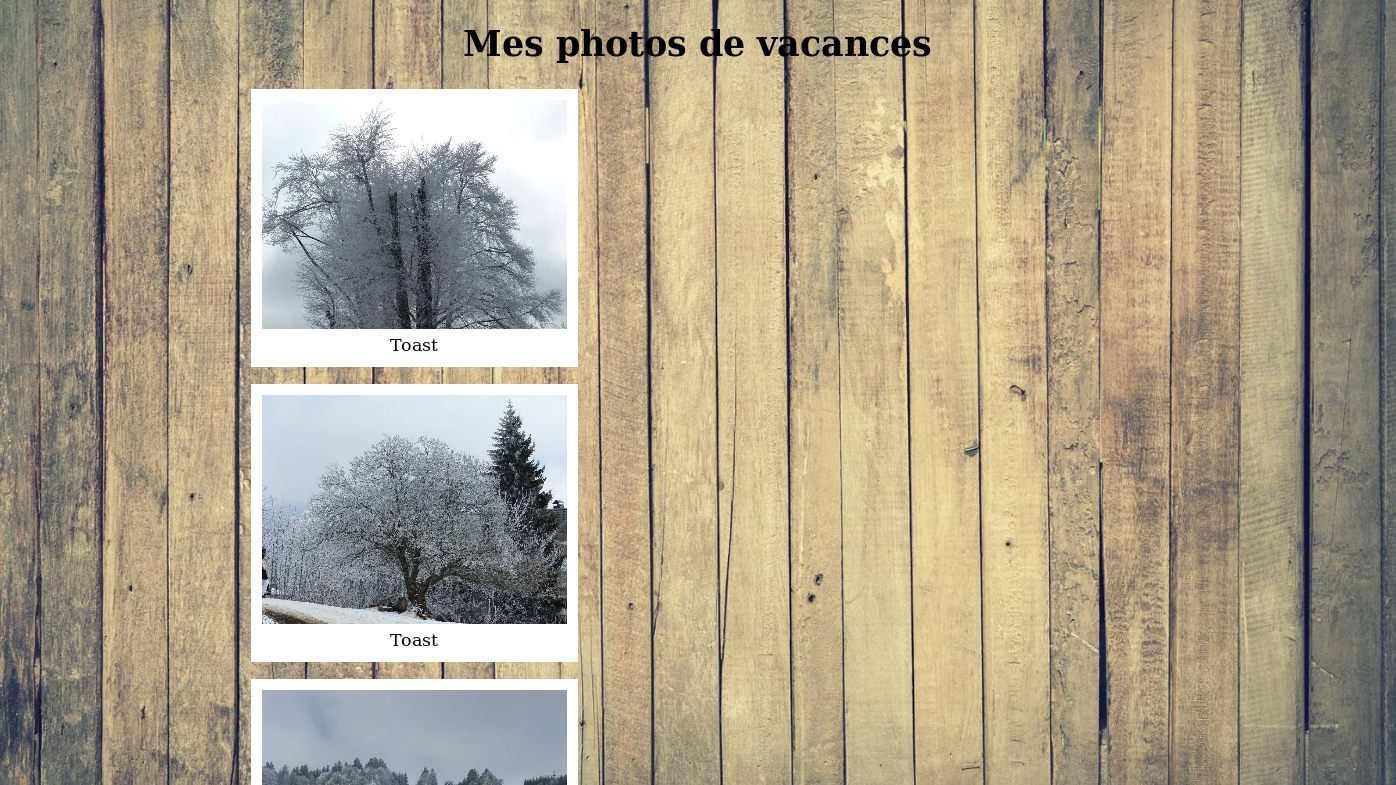
\includegraphics[width=.8\linewidth]{img/screenshot_text-align.png}\end{center}

\subsection{Fonctionnement du TP}
Les solutions de chaque partie de ce TP se trouvent dans le dossier source.
Cependant le but n'est pas que vous copiez la solution sans comprendre, mais
plutôt que vous essayiez de faire comme la solution, et si vous n'y arrivez pas,
la solution est là pour vous débloquer.

\subsection{Un peu de vocabulaire pour mieux se comprendre}
\begin{description}
	\item[Le HTML] Le HTML est le langage utilisé pour écrire des pages web.
		Ici nous allons voir une petite partie du HTML5, la dernière
		version du HTML.
	\item[Le CSS] Le CSS est un langage complémentaire au HTML. Il permet de
		définir comment les différentes parties de la page vont
		s’afficher, en changeant la taille, la couleur et d’autres
		propriétés des éléments de la page. Ici nous utiliserons une
		partie du CSS3.
	\item[Les balises] Les balises permettent de séparer en différentes
		sections les pages HTML. Elles se présentent sous la forme
		suivante : \mintinline{html}{<nom> </nom>} . Ici
		\mintinline{html}{<nom>} ouvre la section, et
		\mintinline{html}{</nom>} la ferme.
	\item[Les attributs] Certaines balises peuvent avoir des attributs. Une
		balise « a » avec un attribut « href » ayant pour valeur
		« gcc.prologin.org » s’écrira de la façon suivante :
		\mintinline{html}{<a href="gcc.prologin.org">Le site de GCC!</a>}
\end{description}

\section{HTML de base}
Pour commencer toutes pages HTML valides, il faut au moins le code suivant :

\begin{minipage}{0.50\textwidth}
\begin{minted}{html}
<!DOCTYPE HTML>
<html>
  <head>
    <meta charset="utf-8">
    <title>Titre de la page</title>
  </head>
  <body>
    Corps de la page
  </body>
</html>
\end{minted}
\end{minipage}
\begin{minipage}{0.50\textwidth}
\begin{minted}{text}
Il s’agit d’une page HTML5
Début du document HTML
  Début de la section « head »
    L'encodage de la page
    Le titre de la page
  Fin de la section « head »
  Début du corps de la page
    Contenu de la page
  Fin du corps de la page
Fin document HTML
\end{minted}
\end{minipage}

La section « head » contient des informations comme le titre de la page, le
thème CSS, ou encore l'encodage, qui nous permet d'écrire des accents dans la
page.

\section{Les balises}
\begin{description}
	\item[\mintinline{html}{<h1>, <h2>, …, <h6>}] Les balises h nous
		permettent d’écrire des titres de section. Le chiffre indique
		le niveau du titre. Généralement, \mintinline{html}{<h1>} est
		le titre de la page, \mintinline{html}{<h2>} le sous-titre,
		etc...
	\item[\mintinline{html}{<header>}] La balise header (entête) va nous
		permettre de mettre le titre, le logo ou encore les différents
		liens de notre site.
	\item[\mintinline{html}{<main>}] La balise main (principal en anglais)
		va contenir le corps de notre page, ici nos photos.
	\item[\mintinline{html}{<figure> et <figcaption>}] Les balises figure
		et figcaption ont pour but d’insérer des illustrations, avec
		possiblement des légendes.
	\item[\mintinline{html}{<footer>}] La balise footer (pied de page) va
		contenir le pied de page, ici notre copyright.
	\item[\mintinline{html}{<img>}] Les balises img vont nous permettre
		d’insérer les photos sur notre page. Pour dire quelle image il
		faut afficher, on a besoin de l’attribut src :

		\mintinline{html}{<img src="img/1.JPG" alt="Un arbre enneigé.">}

		Ces balises sont un peu spéciales : elles n'ont pas besoin
		d'être fermées.

		À noter que pour pour permettre aux mal-voyants de visiter votre
		site, il est obligatoire d’ajouter un attribut alt, contenant
		une description de la photo.
\end{description}

\section{Notre plan de page}
Notre plan de page sera le suivant :
\dirtree{%TODO faire un arbre avec tickz ?
.1 html.
.2 head (voir partie 1).
.2 body.
.3 header.
.4 h1.
.3 main.
.4 figure.
.5 img.
.5 figcaption.
.4 ….
.3 footer.
}
Je vous laisse essayer de créer le document HTML correspondant. Une fois que
vous aurez fait de votre mieux vous pourrez regarder la correction.

Vous devriez arriver au résultat suivant :
\begin{center}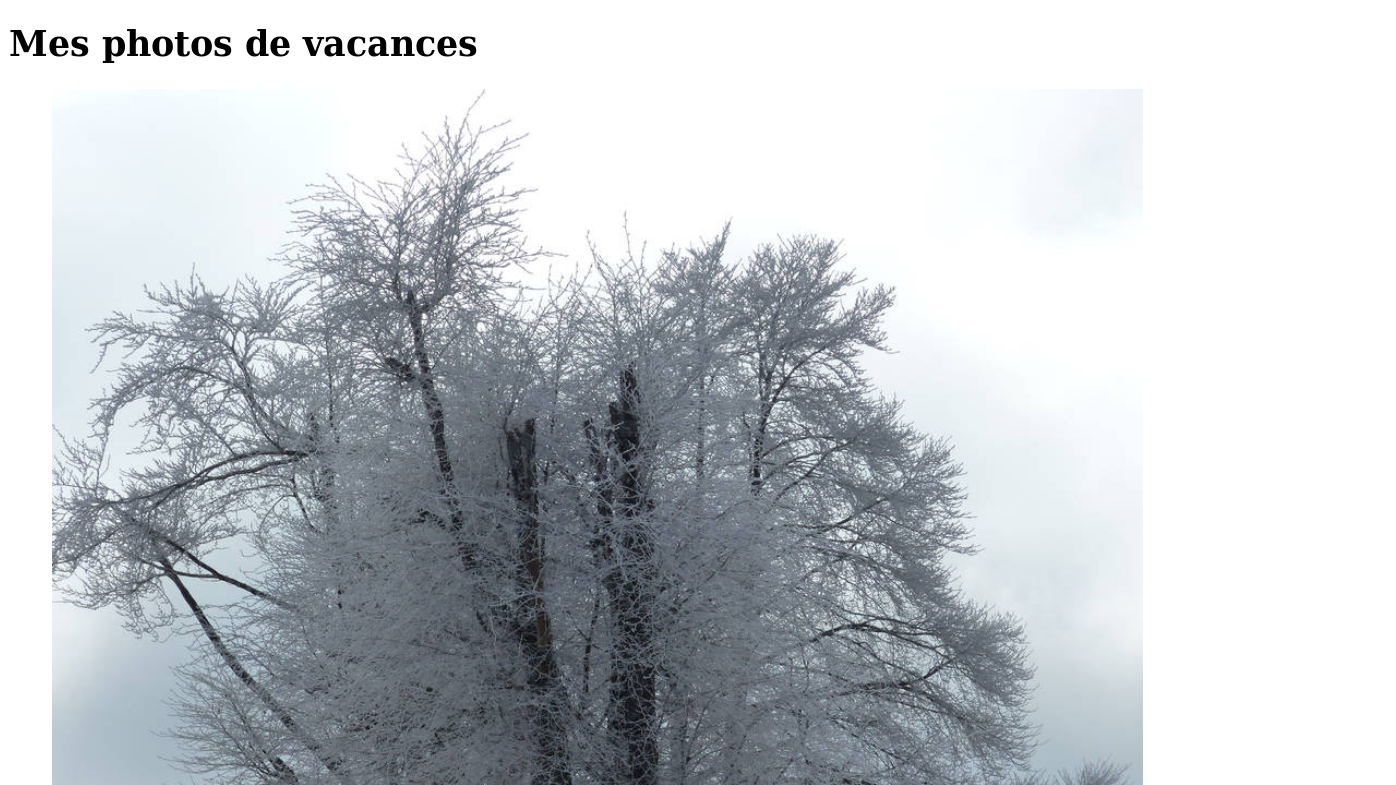
\includegraphics[width=.8\linewidth]{img/screenshot_html.png}\end{center}

\section{Du CSS pour sauver nos yeux}
\subsection{Insérer du CSS dans la page}
Pour insérer du CSS dans une page, nous écrirons notre CSS dans un nouveau
fichier, « style.css », dans le dossier « css ».
Pour dire à notre page HTML d’utiliser ce document CSS, il faut ajouter dans la
balise head la balise suivante :

\mintinline{html}{<link rel="stylesheet" src="css/style.css">}

Comme pour les balises \mintinline{html}{<img>}, il n'est pas nécessaire les
fermer.
\subsection{Écriture du CSS}
Le CSS est un langage basé sur les sélecteurs. Une fois qu’on a sélectionné un
ou plusieurs éléments HTML avec les sélecteurs, on peut modifier son apparence
en changeant ses attributs.
\begin{alltt}
\colorbox{blue!30}{sélecteur} \{
        \colorbox{green!30}{attribut}: \colorbox{red!30}{valeur};
\}
\end{alltt}

\subsubsection{Les unités de mesure}
Tout au long de ce chapitre je vais utiliser différentes unités de mesures. En
voici quelques unes :
\begin{description}
	\item[px] L'unité px permet de définir la taille d'un élément en pixels.
	C'est cette même unité que vous utiliserez dans le projet python.
	\item[\%] Les pourcentages permettent de définir la taille d'un élément
	en fonction de la taille de son élément parent.
\end{description}
\subsubsection{Les sélecteurs}
Nous allons voir 2 types de sélecteurs. Ces différents sélecteurs pourront être
combinés les uns avec les autres pour être plus précis.
\begin{enumerate}
	\item Les sélecteurs d’éléments : Pour sélectionner un type d'élément,
		par exemple les balises img, il suffit d'écrire le nom de la
		balise
	\item Le sélecteur de survol : Pour faire en sorte de détecter la souris
		et changer l’apparence d’un élément quand la souris est dessus,
		il faut rajouter le sélecteur \mintinline{css}{:hover}.
\end{enumerate}
Pour combiner les sélecteurs, il suffit de les juxtaposer. Par exemple pour
sélectionner une image quand elle est survolée, le sélecteur final sera
\mintinline{css}{img:hover}

Pour sélectionner plusieurs éléments différents, il faut séparer les sélecteurs
par une virgule. Par exemple pour appliquer les mêmes propriétés aux éléments h1
ainsi qu'aux éléments img survolés, le sélecteur final sera
\mintinline{css}{h1, img:hover}.

\subsection{Les couleurs}
Les couleurs sont représentées dans un format spécial en CSS. Pour nous aider à
nous y retrouver plus facilement, des outils comme
\href{https://duckduckgo.com/?q=color+picker\&t=ffab\&ia=answer}{le sélecteur de couleur DuckDuckGo} sont là.
\paragraph{}
\begin{center}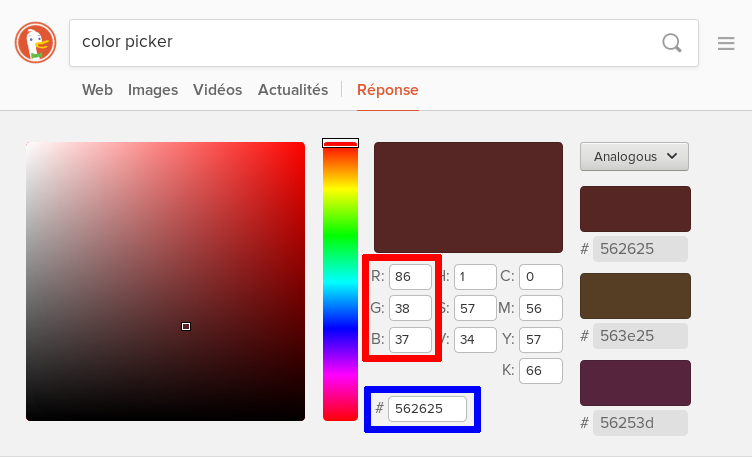
\includegraphics[width=.8\linewidth]{img/ddgo_color_picker.png}\end{center}
Cet outil nous permet de récupérer le code \colorbox{blue!30}{hexadécimal} des
couleurs ainsi que leur représentation \colorbox{red!30}{RGB}. Nous ne verrons
pour l'instant que la représentation hexadécimale.

Le code hexadécimal peut être utilisé tel quel dans le code CSS.
\paragraph{}
Un petit exemple : on va faire en sorte que le texte des figcaptions soit rouge.

\begin{minipage}{0.40\textwidth}
\begin{minted}{css}
figcaption {
  color: #FF0000;
}
\end{minted}
\end{minipage}
\begin{minipage}{0.60\textwidth}
\begin{minted}{text}
On sélectionne les éléments figcaption
  On leur applique une couleur rouge
On ferme le bloc
\end{minted}
\end{minipage}

\subsubsection{Les attributs}
Maintenant que nous avons vu comment sélectionner les balises que nous
souhaitons modifier, nous allons voir comment changer leur attributs pour
modifier leur taille, leur position et leurs couleurs.

\paragraph{color}
L'attribut color permet de changer la couleur du texte. Elle prend en argument
une couleur, qui sera appliqué à cet élément ainsi qu'à tout ses sous-éléments.

\paragraph{background}
L'attribut background permet quand à lui de changer la couleur de fond d'un
élément.

\begin{minipage}{0.40\textwidth}
\begin{minted}{css}
figure {
  background: #008AFF;
}
\end{minted}
\end{minipage}
\begin{minipage}{0.60\textwidth}
\begin{minted}{text}
On sélectionne les élements figure
  On leur applique un fond couleur cyan
Fin du bloc
\end{minted}
\end{minipage}

L'attribut background peut aussi définir une image de fond, par exemple, le site
final utilise le code suivant :

\begin{minipage}{0.40\textwidth}
\begin{minted}{css}
html {
  background:
      fixed
      center / cover
      url('../img/fond.jpg')
    ;
}
\end{minted}
\end{minipage}
\begin{minipage}{0.60\textwidth}
\begin{minted}{text}
On sélectionne le document HTML entier
  On va modifier le fond
      Le fond ne bougera pas avec la page
      L'image sera centrée, et couvrira tout
      L'image qu'on veut afficher
    Fin de la modification du fond
On ferme le bloc
\end{minted}
\end{minipage}

Ici nous ne changerons que 3 fonds : le fond de la page, le fond des figures et
le fond du footer. Vous devrez appliquer un fond blanc aux éléments figure et
footer, et copier le code pour le fond de la page afin d'obtenir ce résultat :
\begin{center}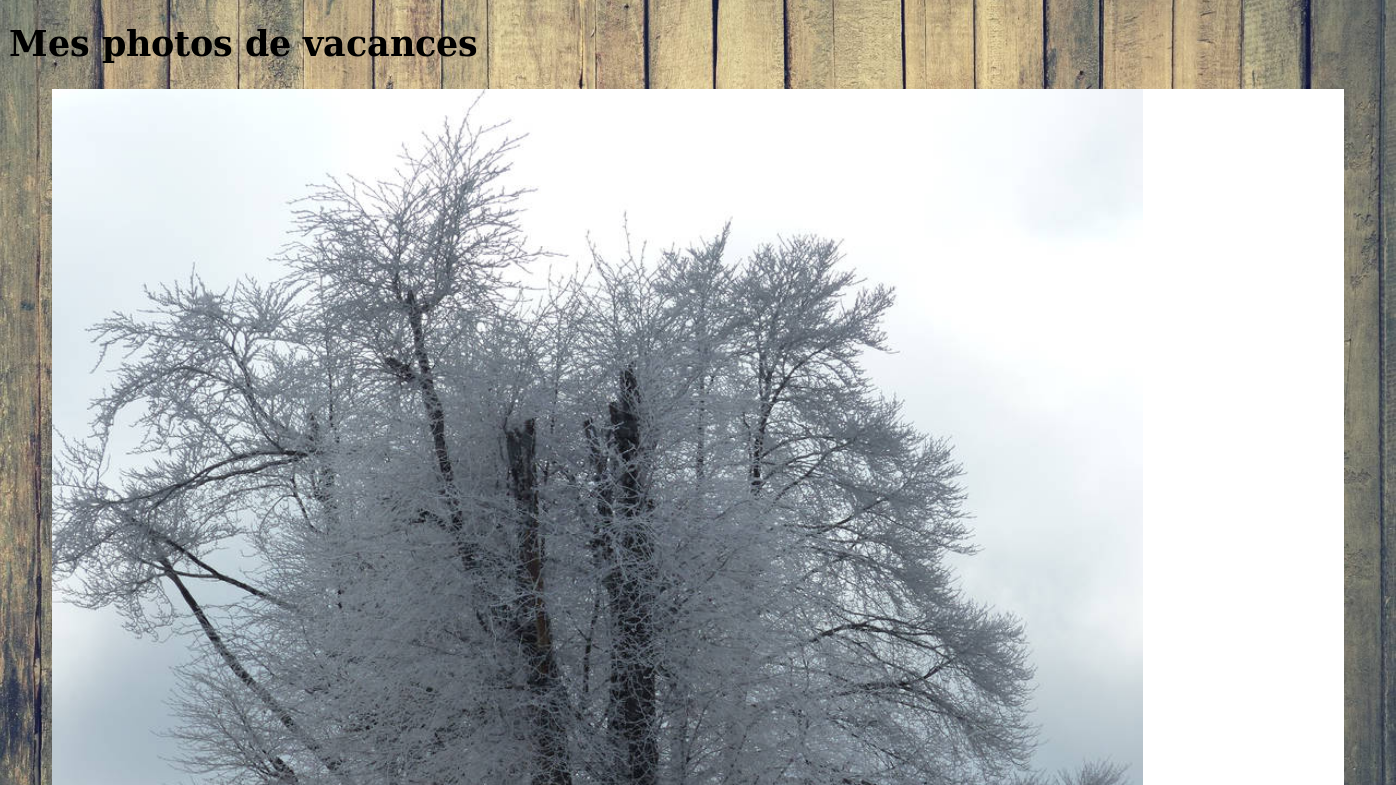
\includegraphics[width=.8\linewidth]{img/screenshot_background.png}\end{center}

\paragraph{width et height}
Les attributs width (largeur) et height (hauteur) permettent de faire en sorte
qu'un élément ait une certaine taille.

Il existe aussi min-height, max-height,
et les mêmes attributs pour width, qui permettent de définir des valeurs minimum
et maximum pour les éléments.

Par exemple, dans le code final, l'élément main contient ces attributs :

\begin{minipage}{0.35\textwidth}
\begin{minted}{css}
main {
  width: 900px;
  max-width: 80%;
}
\end{minted}
\end{minipage}
\begin{minipage}{0.65\textwidth}
\begin{minted}{text}

largeur de base de 900px
si la fenêtre est trop petite, 80% max

\end{minted}
\end{minipage}

Pour le moment nous ne changerons que 3 largeurs : la largeur de main, que vous
avez eu en exemple, la largeur de figure que nous définirons à 280px, et enfin
la largeur des éléments img dans des figure, que nous définirons à 100\%.
\begin{center}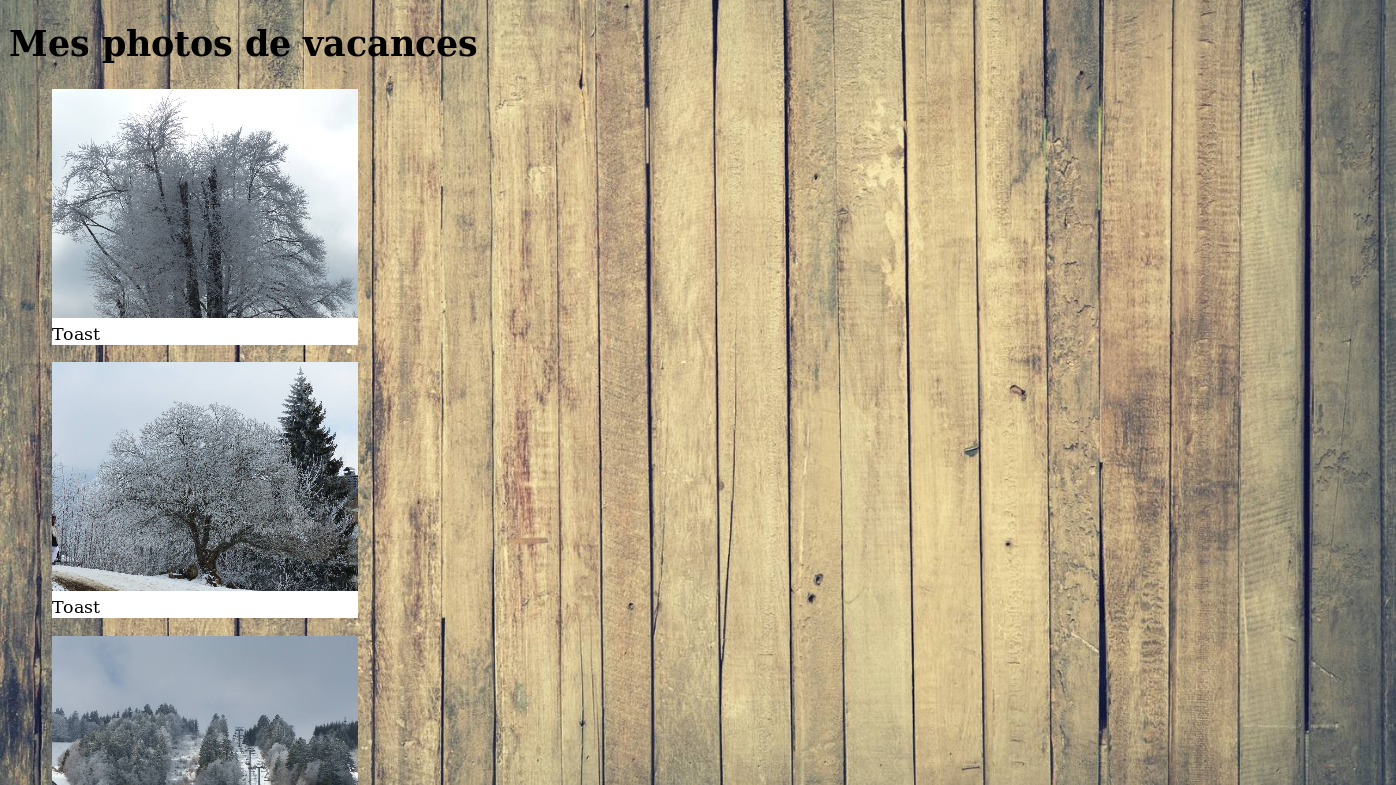
\includegraphics[width=.8\linewidth]{img/screenshot_width.png}\end{center}

\paragraph{padding et margin}
Ces deux attributs permettent de modifier la "marge" et le "remplissage" des
éléments. Pour mieux comprendre à quoi correspondent la marge et le remplissage,
voici un diagramme réalisé par les contributeurs Mozilla, disponible
\href{https://developer.mozilla.org/fr/docs/Apprendre/CSS/Introduction_%C3%A0_CSS/Le_mod%C3%A8le_de_bo%C3%AEte}{à l'addresse suivante}.
\begin{center}
\includegraphics[width=.8\linewidth]{img/box_model.png}\end{center}

Ici, j'utilise des marges et du padding pour le pied de page :
\begin{minted}{css}
footer {
    ...
    padding: 20px;
    margin-top: 30px;
    ...
}
\end{minted}
Ce code permet de rajouter du remplissage tout autours du texte du pied de page,
et de rajouter une marge afin de séparer les photos du pied de page.

-top permet de n’appliquer la marge que sur le coté supérieur du pied de page.
Il existe aussi -left (gauche) -right (droite) et -bottom (bas).

Les marges peuvent aussi être utilisées pour centrer un élément sur la page :
\begin{minted}{css}
main {
    ...
    margin-left: auto;
    margin-right: auto;
}
\end{minted}
En indiquant que la marge gauche et droite doivent être calculées
automatiquement, l'élément se retrouve centré horizontalement.

Ici vous devrez:
\begin{enumerate}
	\item Mettre les marges de l'élément body à 0
	\item Centrer horizontalement l'élément main (comme dans l'exemple)
	\item Ajouter un padding de 10px aux éléments figure
	\item Ajouter un padding de 20px au footer, et aussi un margin-top de
	30px
\end{enumerate}
\begin{center}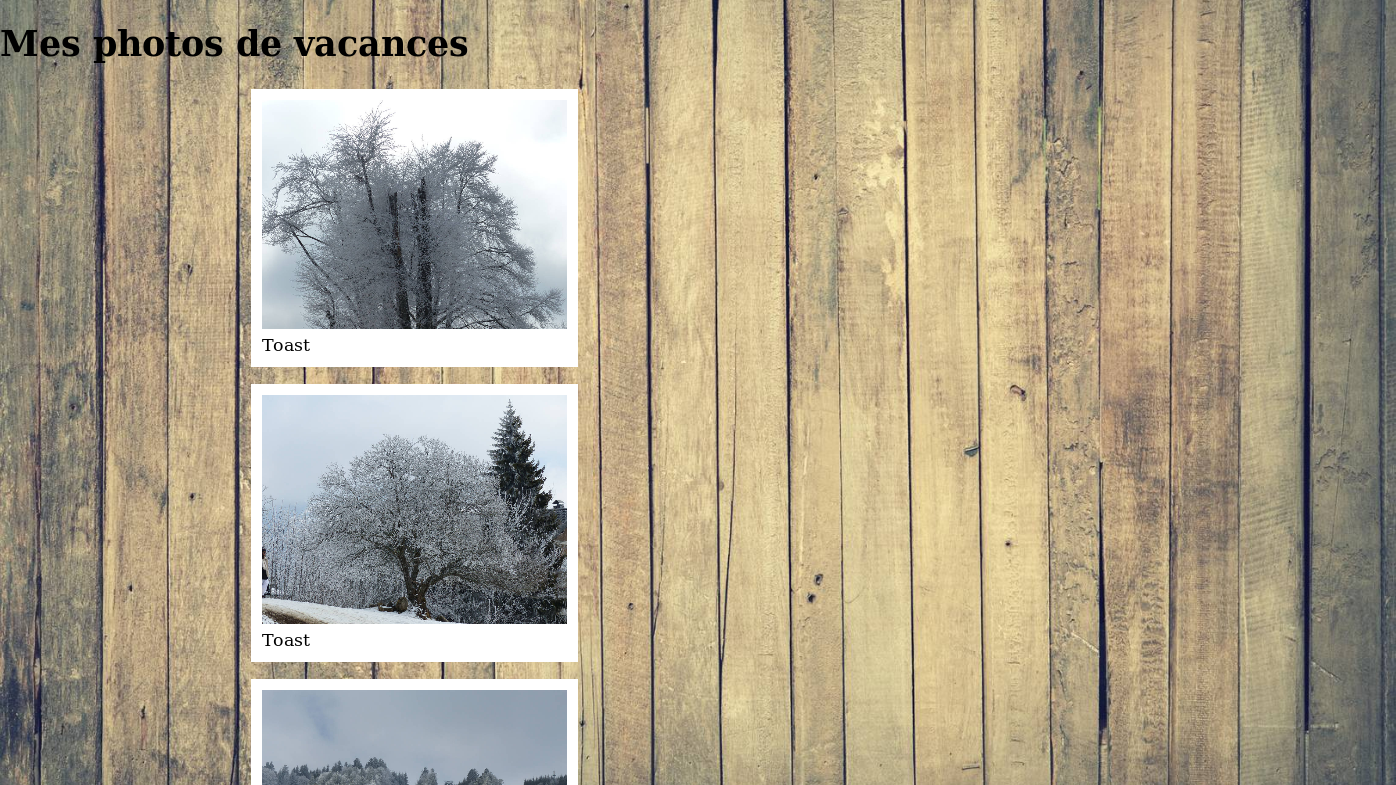
\includegraphics[width=.8\linewidth]{img/screenshot_padding.png}\end{center}

\paragraph{text-align}
L'attribut text-align permet de choisir comment sera aligné le texte. Par défaut
text-align a pour valeur "left" car en français le texte va de gauche à droite.

Ici, vous ajouterez "text-align: center" à l'élément header, au footer et aux
éléments figure figcaption.
\begin{center}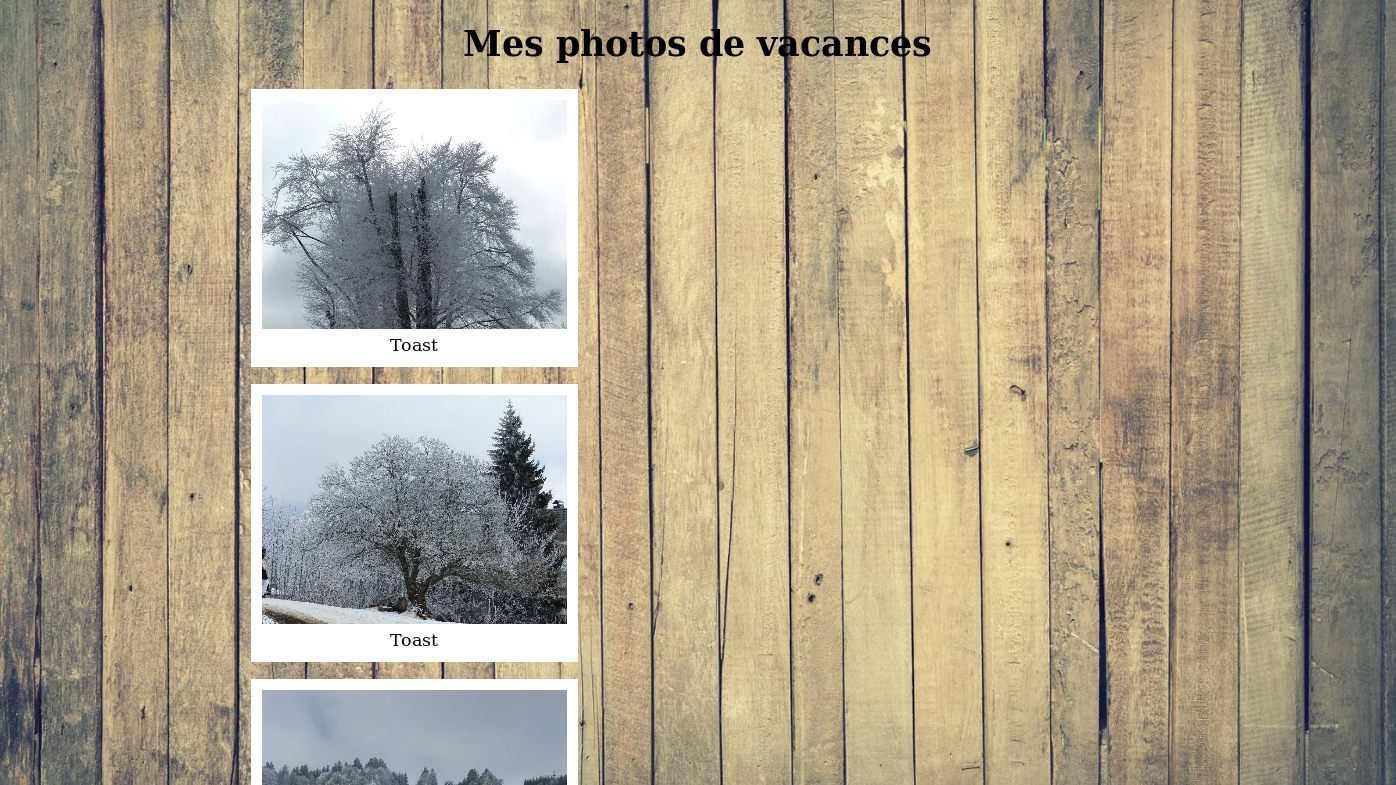
\includegraphics[width=.8\linewidth]{img/screenshot_text-align.png}\end{center}

\section{La fin! (?)}
Félicitations, vous avez terminé ce TP !

Pour aller plus loin, une partie bonus existe, demandez aux organisateurs de
vous la donner !
